\documentclass{ctexrep}
\usepackage[T1]{fontenc}
\usepackage[a4paper,top=1.5cm,bottom=1.5cm,left=2cm,right=2cm,marginparwidth=1.75cm]{geometry}
\usepackage{mathtools}
\usepackage{tikz}
\usepackage{booktabs}
\usepackage{caption}
\usepackage{outlines}
\usepackage{graphicx}
\usepackage{float}
\usepackage{amsthm}
\usepackage{tabu}
\usepackage{minted}
\usepackage[colorlinks=false, allcolors=blue]{hyperref}
\usepackage{cleveref}
\usepackage{pdfpages}
\usepackage{underscore}
\usepackage{wrapfig}
\usepackage{subcaption}
\usepackage{pgfplots}
\usepackage{multicol}
\renewcommand{\tableautorefname}{表}
\DeclarePairedDelimiter{\set}{\{}{\}}
\DeclarePairedDelimiter{\paren}{(}{)}
\graphicspath{ {./images/} }
\crefname{equation}{方程}{方程}
\crefname{algorithm}{算法}{算法}
\crefname{lemma}{引理}{引理}
\crefname{table}{表}{表}
\crefname{figure}{图}{图}
\newcounter{fullrefcounter}
\newcommand*{\fullref}[1]{%
\addtocounter{fullrefcounter}{1}%
\label{--ref-\thefullrefcounter}%
\ifthenelse{\equal{\getpagerefnumber{--ref-\thefullrefcounter}}{\getpagerefnumber{#1}}}
  {
    \hyperref[{#1}]{\Cref*{#1} \nameref*{#1}}
  }
  {% false case
    \hyperref[{#1}]{第 \pageref*{#1} 页 \Cref*{#1} \nameref*{#1}}
  }
}
% \makeatother

\newcommand{\expfig}[2]{
    \begin{subfigure}[b]{0.3\textwidth}
        \centering
        \begin{tikzpicture}
            \begin{axis}[
                width=\textwidth,
                height=\textwidth,
                xmode=log,
                log basis x={2},
            ]
            \addplot+[] coordinates {
                #1
            };
            \addplot[] coordinates {
                #1
            };
            \end{axis}
        \end{tikzpicture}
        \caption{#2}
    \end{subfigure}%
}
\newcommand{\expfigstr}[2]{
    \begin{subfigure}[b]{0.3\textwidth}
        \centering
        \begin{tikzpicture}
            \begin{axis}[
                width=\textwidth,
                height=\textwidth,
                symbolic x coords={l, f, r},
            ]
            \addplot+[ybar] coordinates {
                #1
            };
            \addplot[ybar] coordinates {
                #1
            };
            \end{axis}
        \end{tikzpicture}
        \caption{#2}
    \end{subfigure}%
}
\newcommand{\figroup}[7]{
    \begin{figure}[htp]
        \centering
        \expfig{#3}{test-fmath}
        \expfig{#4}{test-llong}
        \expfig{#5}{test-lswlr}

        \vspace{1em}

        \expfig{#6}{test-math}
        \expfig{#7}{test-printf}
        \caption{#1}
        \label{#2}
    \end{figure}
}
\newcommand{\figroupstr}[7]{
    \begin{figure}[htp]
        \centering
        \expfigstr{#3}{test-fmath}
        \expfigstr{#4}{test-llong}
        \expfigstr{#5}{test-lswlr}

        \vspace{1em}

        \expfigstr{#6}{test-math}
        \expfigstr{#7}{test-printf}
        \caption{#1}
        \label{#2}
    \end{figure}
}


\ctexset{
    chapter = {
        name = {第,部分}
    },
    section = {
        titleformat = \raggedright,
        % name = {,},
        % number = \chinese{section}、
    },
    paragraph = {
        runin = false
    },
    today = small,
    figurename = 图,
    contentsname = 目录,
    tablename = 表,
}

\newmintinline[gas]{gas}{}

\begin{document}

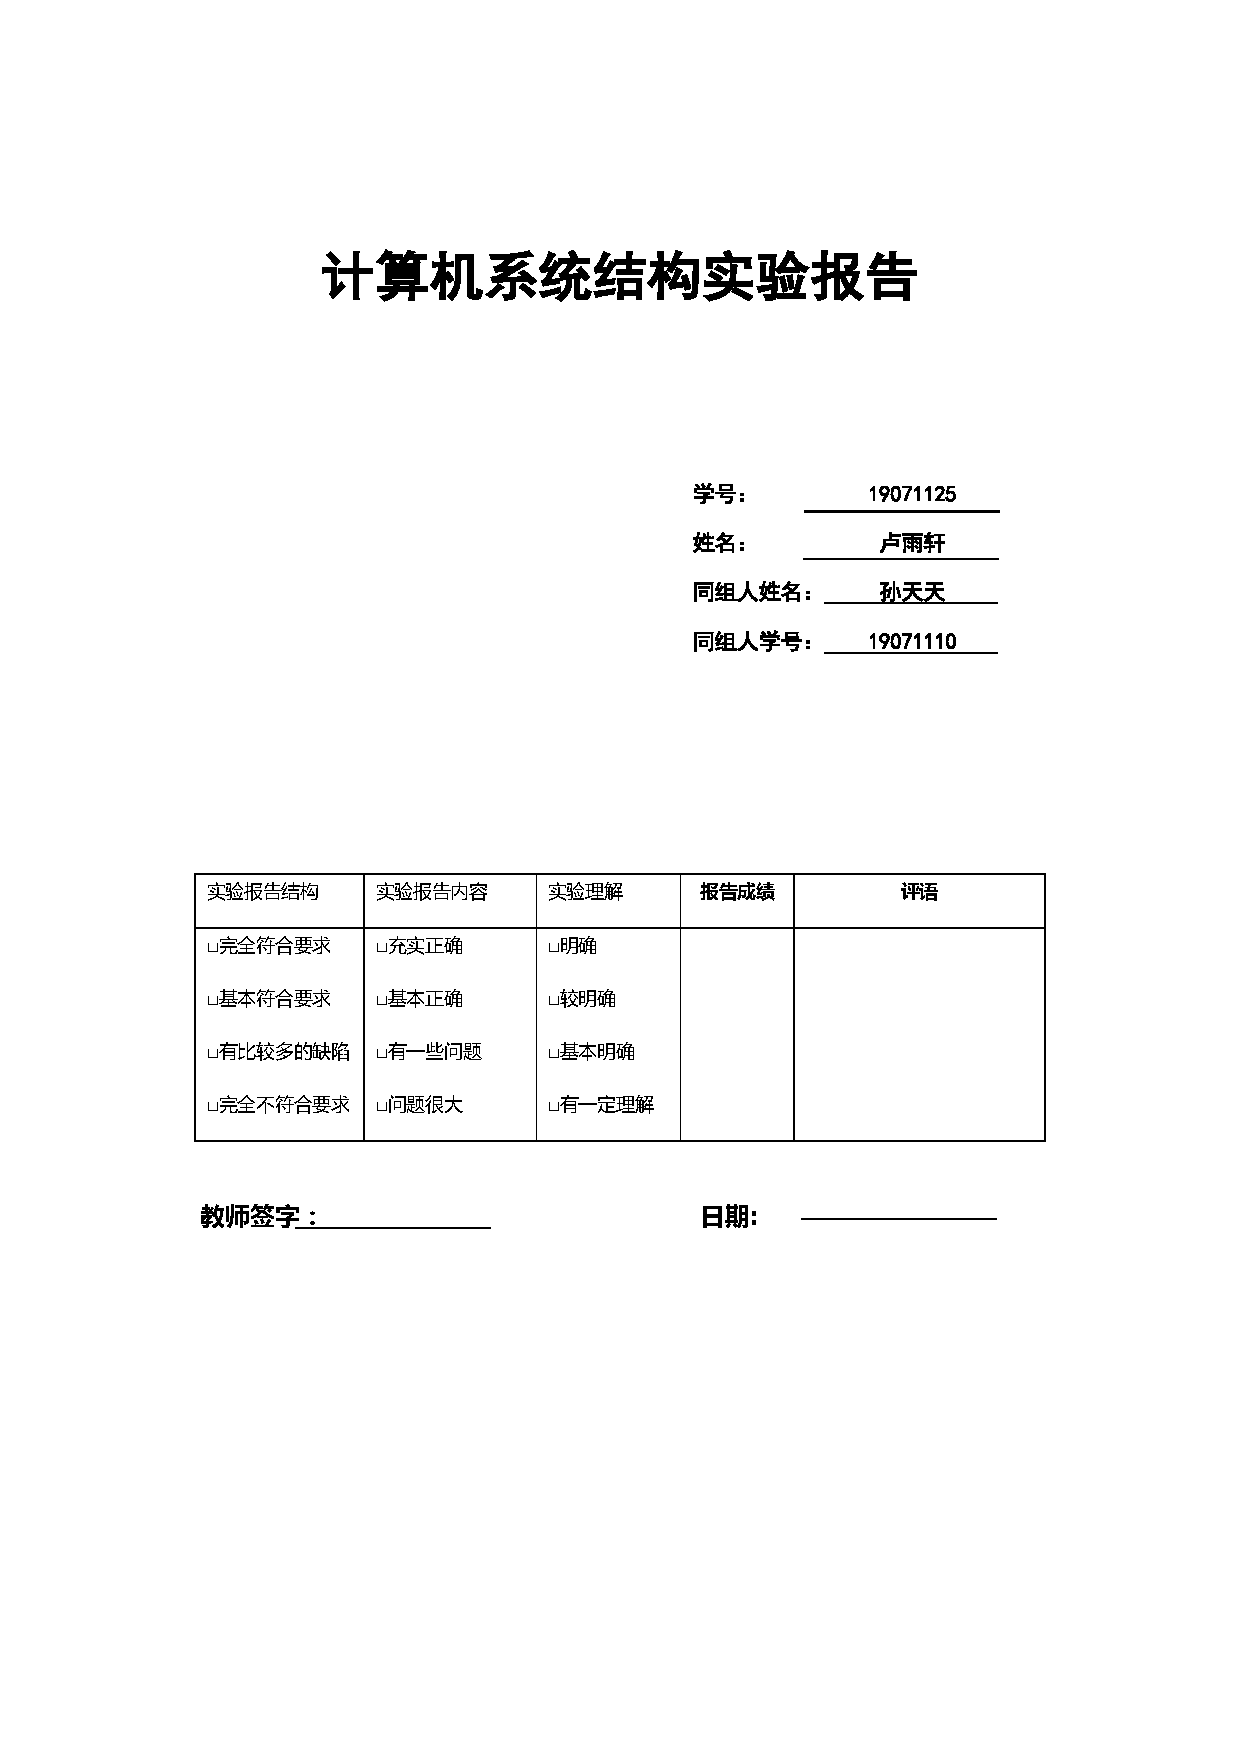
\includepdf{cover.pdf}
\tableofcontents

\chapter{流水线、指令调度与循环展开}

\section{流水线中的相关}

\subsection{实验目的}
\begin{outline}[enumerate]
    \1 熟练掌握WinMIPS64模拟器的操作和使用,熟悉MIPS指令集结构及其特点;
    \1 加深对计算机流水线基本概念的理解;
    \1 进一步了解MIPS基本流水线各段的功能以及基本操作;
    \1 加深对数据相关、结构相关的理解,了解这两类相关对CPU 性能的影响;
    \1 了解解决数据相关的方法,掌握如何使用定向技术来减少数据相关带来的暂停。
\end{outline}
\subsection{实验内容与步骤}
\begin{outline}[enumerate]
    \1 用WinMIPS64模拟器执行三个程序,分别以步进、连续的方式运行程序,观察程序在流水线中的执行情况,观察CPU 中寄 存器和存储器的内容。熟练掌握WinMIPS64的操作和使用。
123 123
    \1 用WinMIPS64运行程序test_for.s,通过模拟找出存在资源相关的指令对以及导致资源 相关的部件;记录由资源相关引起的暂停时钟周期数,计算暂停时钟周期数占总执行周期数 的百分比;论述资源相关对CPU性能的影响,讨论解决资源相关的方法。

    \1 在不采用定向技术的情况下(去掉Configuration菜单中Enable Forwarding选项前的 勾选符),用WinMIPS64运行程序sum.s和test_for.s。记录数据相关引起的暂停时钟周期数以 及程序执行的总时钟周期数,计算暂停时钟周期数占总执行周期数的百分比。在采用定向技 术的情况下(勾选Enable Forwarding),用WinMIPS64再次运行程序sum.s和test_for.s。重复 上述3中的工作,并计算采用定向技术后性能提高的倍数。
\end{outline}
\subsection{实验结果}
\subsubsection{test_for.s的数据相关}
test_for.s的代码为:
\begin{minted}[linenos]{gas}
.data  
a: .space 48  
b: .word 10,11,12,13,0,1  
c: .word 1,2,3,4,5,6  
    
.text 
;initialize registers  
daddi r1,r0,a  
daddi r2,r0,b  
daddi r3,r0,c  
daddi r4,r0,6  
Loop: lw r5,0(r1) ; element of a 
    lw r6,0(r2) ; element of b 
    lw r7,0(r3) ; element of c          
    dadd r8,r5,r6 ; a[i] + b[i]          
    dadd r9,r7,r8 ; a[i] = a[i] + b[i] + c[i];            
    sw r9,0(r1) ; store value in a[i]            
    daddi r1,r1,8 ; increment memory pointers            
    daddi r2,r2,8            
    daddi r3,r3,8            
    daddi r4,r4,-1 ; i++            
    bnez r4,Loop              
end: halt
\end{minted}

\begin{wrapfigure}[4]{r}{.4\linewidth}
    \vspace{-10cm}
    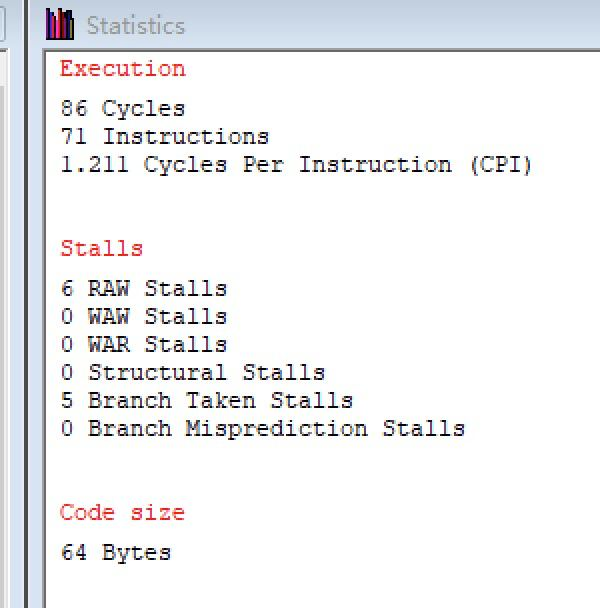
\includegraphics[width=\linewidth]{test_for.s_result.jpeg}
    \caption{test_for.s 运行结果} \label{fig:test-for-result}
\end{wrapfigure}
运行结果见\fullref{fig:test-for-result}。可以看到,程序一共运行了86周期,其中有6次数据相关(Read after Write Stall)的暂停,占总时钟周期的7\%。数据相关会导致CPU空置,会显著影响性能。

\begin{wrapfigure}[6]{r}{.4\linewidth}
    \vspace{-4cm}
    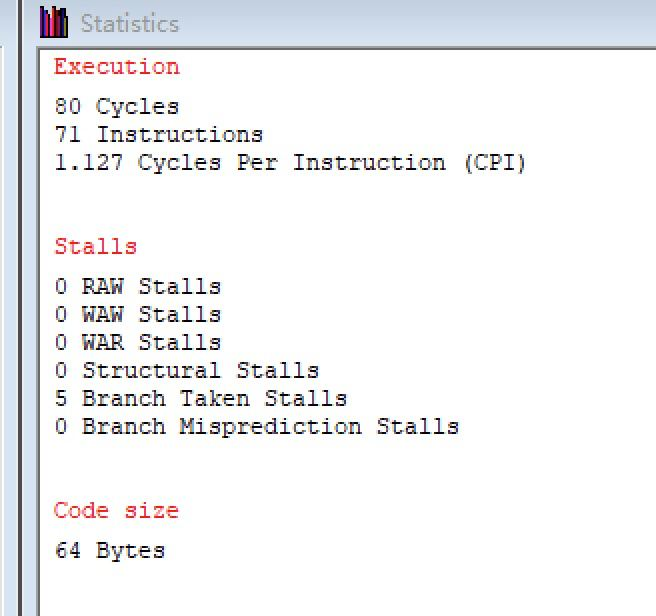
\includegraphics[width=\linewidth]{test_for.s_fixed.jpeg}
    \caption{test_for.s 修改后运行结果} \label{fig:test-for-fixed}
\end{wrapfigure}
程序中第21和22行对 \gas|r4| 寄存器存在先写后读的数据相关。只需要将21行和20行交换位置计即可解决。修改后的运行结果见\fullref{fig:test-for-fixed}。

\subsubsection{定向技术对程序运行的影响}

关闭定向技术之后,分别运行sum.s和test_for.s,发现分别有4和42个先读后写的数据相关引起的暂停,分别占总周期数量 $6 / 86 = 30.8 \%$ 与 $42 / 122 = 34.4\%$。重新启用后运行,发现分别有1和个6个先读后写的暂停,性能分别提高了$ 13 / 10 = 1.3 $与$122 / 86 = 1.418$ 倍。程序运行结果见\fullref{fig:forward}。

\begin{figure}[htp]
    \centering
    \begin{subfigure}{.4\linewidth}
        \centering
        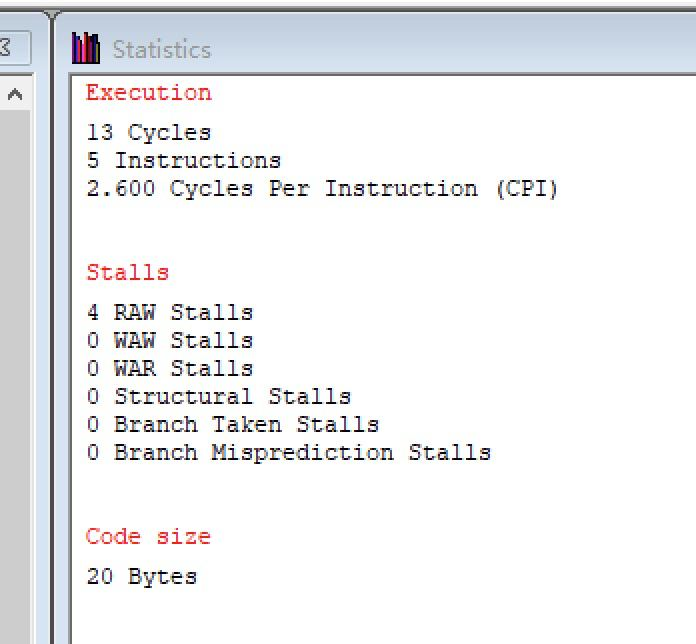
\includegraphics[width=\linewidth]{sum.s_without_forwarding.jpeg}
        \caption{sum.s 不启用forwarding运行结果}
    \end{subfigure}
    \begin{subfigure}{.4\linewidth}
        \centering
        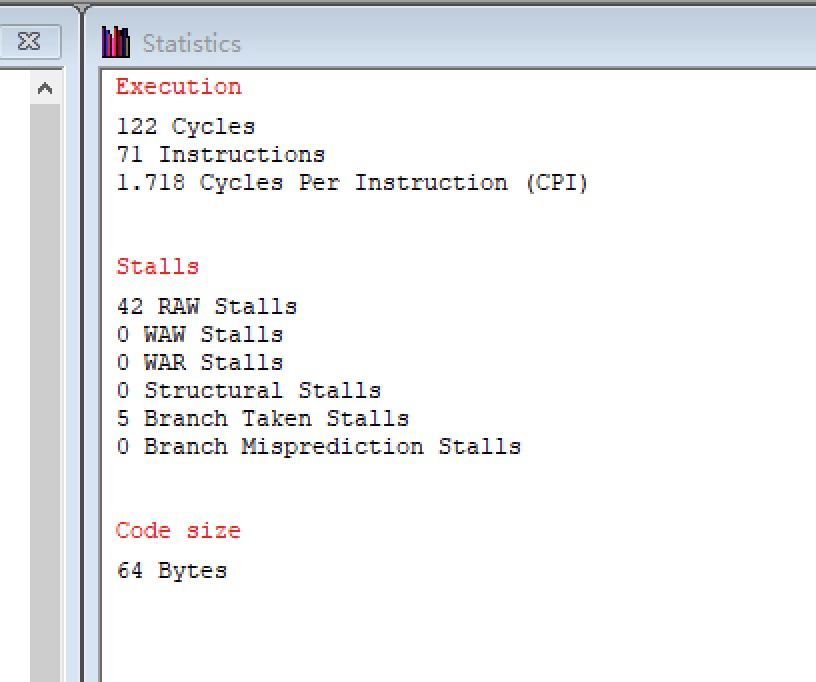
\includegraphics[width=\linewidth]{test_for.s_without_forwarding.jpeg}
        \caption{test_for.s 不启用forwarding运行结果}
    \end{subfigure}

    
    \begin{subfigure}{.4\linewidth}
        \centering
        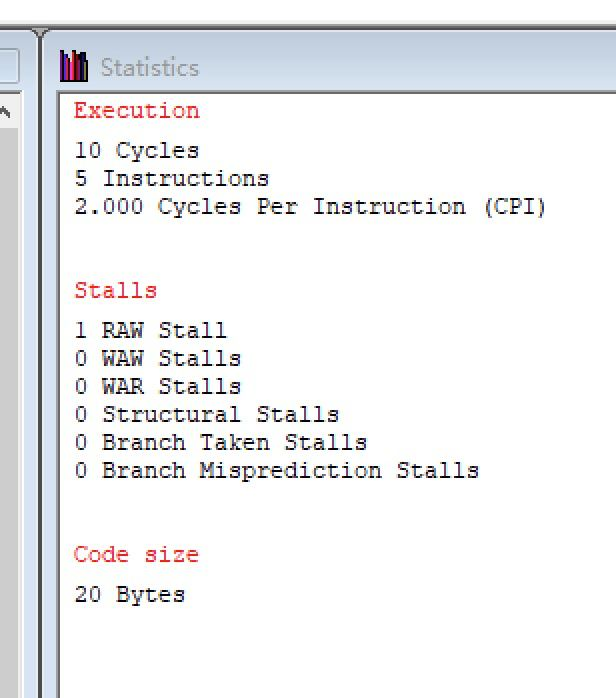
\includegraphics[width=\linewidth]{sum.s_with_forwarding.jpeg}
        \caption{sum.s 启用forwarding运行结果}
    \end{subfigure}
    \begin{subfigure}{.4\linewidth}
        \centering
        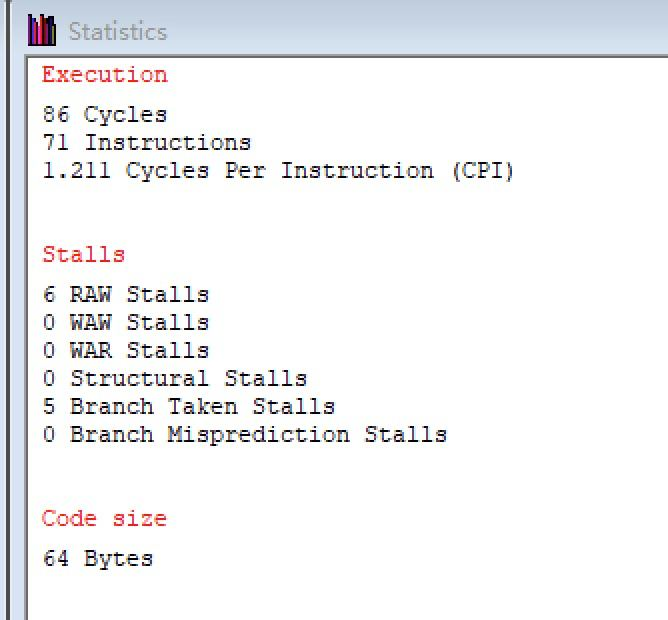
\includegraphics[width=\linewidth]{test_for.s_with_forwarding.jpeg}
        \caption{test_for.s 启用forwarding运行结果}
    \end{subfigure}
    \caption{启用和关闭Forwarding对程序运行的影响}
    \label{fig:forward}
\end{figure}

\section{循环展开和指令调度}
\subsection{实验目的}
\begin{outline}[enumerate]
    \1 加深对循环级并行性、指令调度技术、循环展开技术以及寄存器换名技术的理解
    \1 熟悉用指令调度技术来解决流水线中的数据相关的方法;
    \1 了解循环展开、指令调度等技术对 CPU 性能的改进。
\end{outline}
\subsection{实验步骤}

\begin{outline}[enumerate]
    \1 用指令调度技术解决流水线中的结构相关与数据相关
        \2 用DLX汇编语言编写代码文件*.s,程序中应包括数据相关与结构相关(假设:加法、乘法、除法部件各有2个,延迟时间都是3个时钟周期)
        \2 通过Configuration 菜单中的“Floatingpointstages” 选项,把加法、乘法、除法部件的个数设置为2个,把延迟都设置为3个时钟周期;
        \2 用WinDLX/ WinMIPS64运行程序。记录程序执行过程中各种相关发生的次数、发生相关的指令组合,以及程序执行的总时钟周期数;
        \2 采用指令调度技术对程序进行指令调度,消除相关;
        \2 用WinDLX/ WinMIPS64运行调度后的程序,观察程序在流水线中的执行情况,记录程序执行的总时钟周期数;
        \2 根据记录结果,比较调度前和调度后的性能。论述指令调度对于提高CPU性能的意义。
    \1 用循环展开、寄存器换名以及指令调度提高性能
        \2 用DLX 汇编语言编写代码文件*.s,程序中包含一个循环次数为4 的整数倍的简单循 环;
        \2 用WinDLX 运行该程序。记录执行过程中各种相关发生的次数以及程序执行的总时钟 周期数;
        \2 将循环展开3次,将4个循环体组成的代码代替原来的循环体,并对程序做相应的修改。 然后对新的循环体进行寄存器换名和指令调度;
        \2 用WinDLX/ WinMIPS64运行修改后的程序,记录执行过程中各种相关发生的次数以及 程序执行的总时钟周期数;
        \2 根据记录结果,比较循环展开、指令调度前后的性能。
\end{outline}

\subsection{实验结果}
\subsubsection{指令调度技术解决结构相关与数据相关}

实验中使用的程序为:

\begin{multicols}{2}
\begin{minted}[linenos,breaklines=true]{gas}
.data
title:  .asciiz "Test instructions reordering\n"

CONTROL: .word32 0x10000
DATA:    .word32 0x10008

.text

lwu r21,CONTROL(r0)
lwu r22,DATA(r0)

daddi r1, r0, 0
daddi r2, r0, 1
daddi r3, r0, 2
daddi r4, r0, 3
daddi r5, r0, 4
daddi r6, r0, 5
daddi r7, r0, 6
daddi r8, r0, 7

; calculate (r1+r2) * r3 * r4 + r5 * r6 * r7 * r8
dadd r11, r1, r2
dmulu r11, r11, r3
dmulu r11, r11, r4
dmulu r12, r5, r6
dmulu r13, r7, r8
dmulu r12, r12, r13
dadd r11, r11, r12

daddi r24,r0,1      ; integer output
sd r11,(r22)        ; should be 1562
sd r24,(r21)

halt
\end{minted}
\end{multicols}

程序首先给 \gas{r1} \textasciitilde \gas{r8} 寄存器赋初值,接着计算表达式\mintinline{text}{(r1+r2) * r3 * r4 + r5 * r6 * r7 * r8} 的值,最终输出计算结果。

程序运行过程中,在第24和25行之间有对 \gas{r11} 寄存器的先读后写的数据相关。通过指令调度技术,将第26到27行移到24和25行中间,即可解决数据相关:

\begin{multicols}{2}
\begin{minted}[linenos,breaklines=true]{gas}
.data
title:  .asciiz "Test instruction reordering\n"

CONTROL: .word32 0x10000
DATA:    .word32 0x10008

.text

lwu r21,CONTROL(r0)
lwu r22,DATA(r0)

daddi r1, r0, 0
daddi r2, r0, 1
daddi r3, r0, 2
daddi r4, r0, 3
daddi r5, r0, 4
daddi r6, r0, 5
daddi r7, r0, 6
daddi r8, r0, 7

# calculate (r1+r2) * r3 * r4 + r5 * r6 * r7 * r8
dadd r11, r1, r2
dmulu r11, r11, r3
dmulu r12, r5, r6
dmulu r13, r7, r8
dmulu r11, r11, r4
dmulu r12, r12, r13
dadd r11, r11, r12

# dadd r8, r6, r7

daddi r24,r0,1      ; integer output
sd r11,(r22)  # should be 1562
sd r24,(r21)

halt
\end{minted}
\end{multicols}

\begin{figure}
    \centering
    \begin{subfigure}{.8\linewidth}
        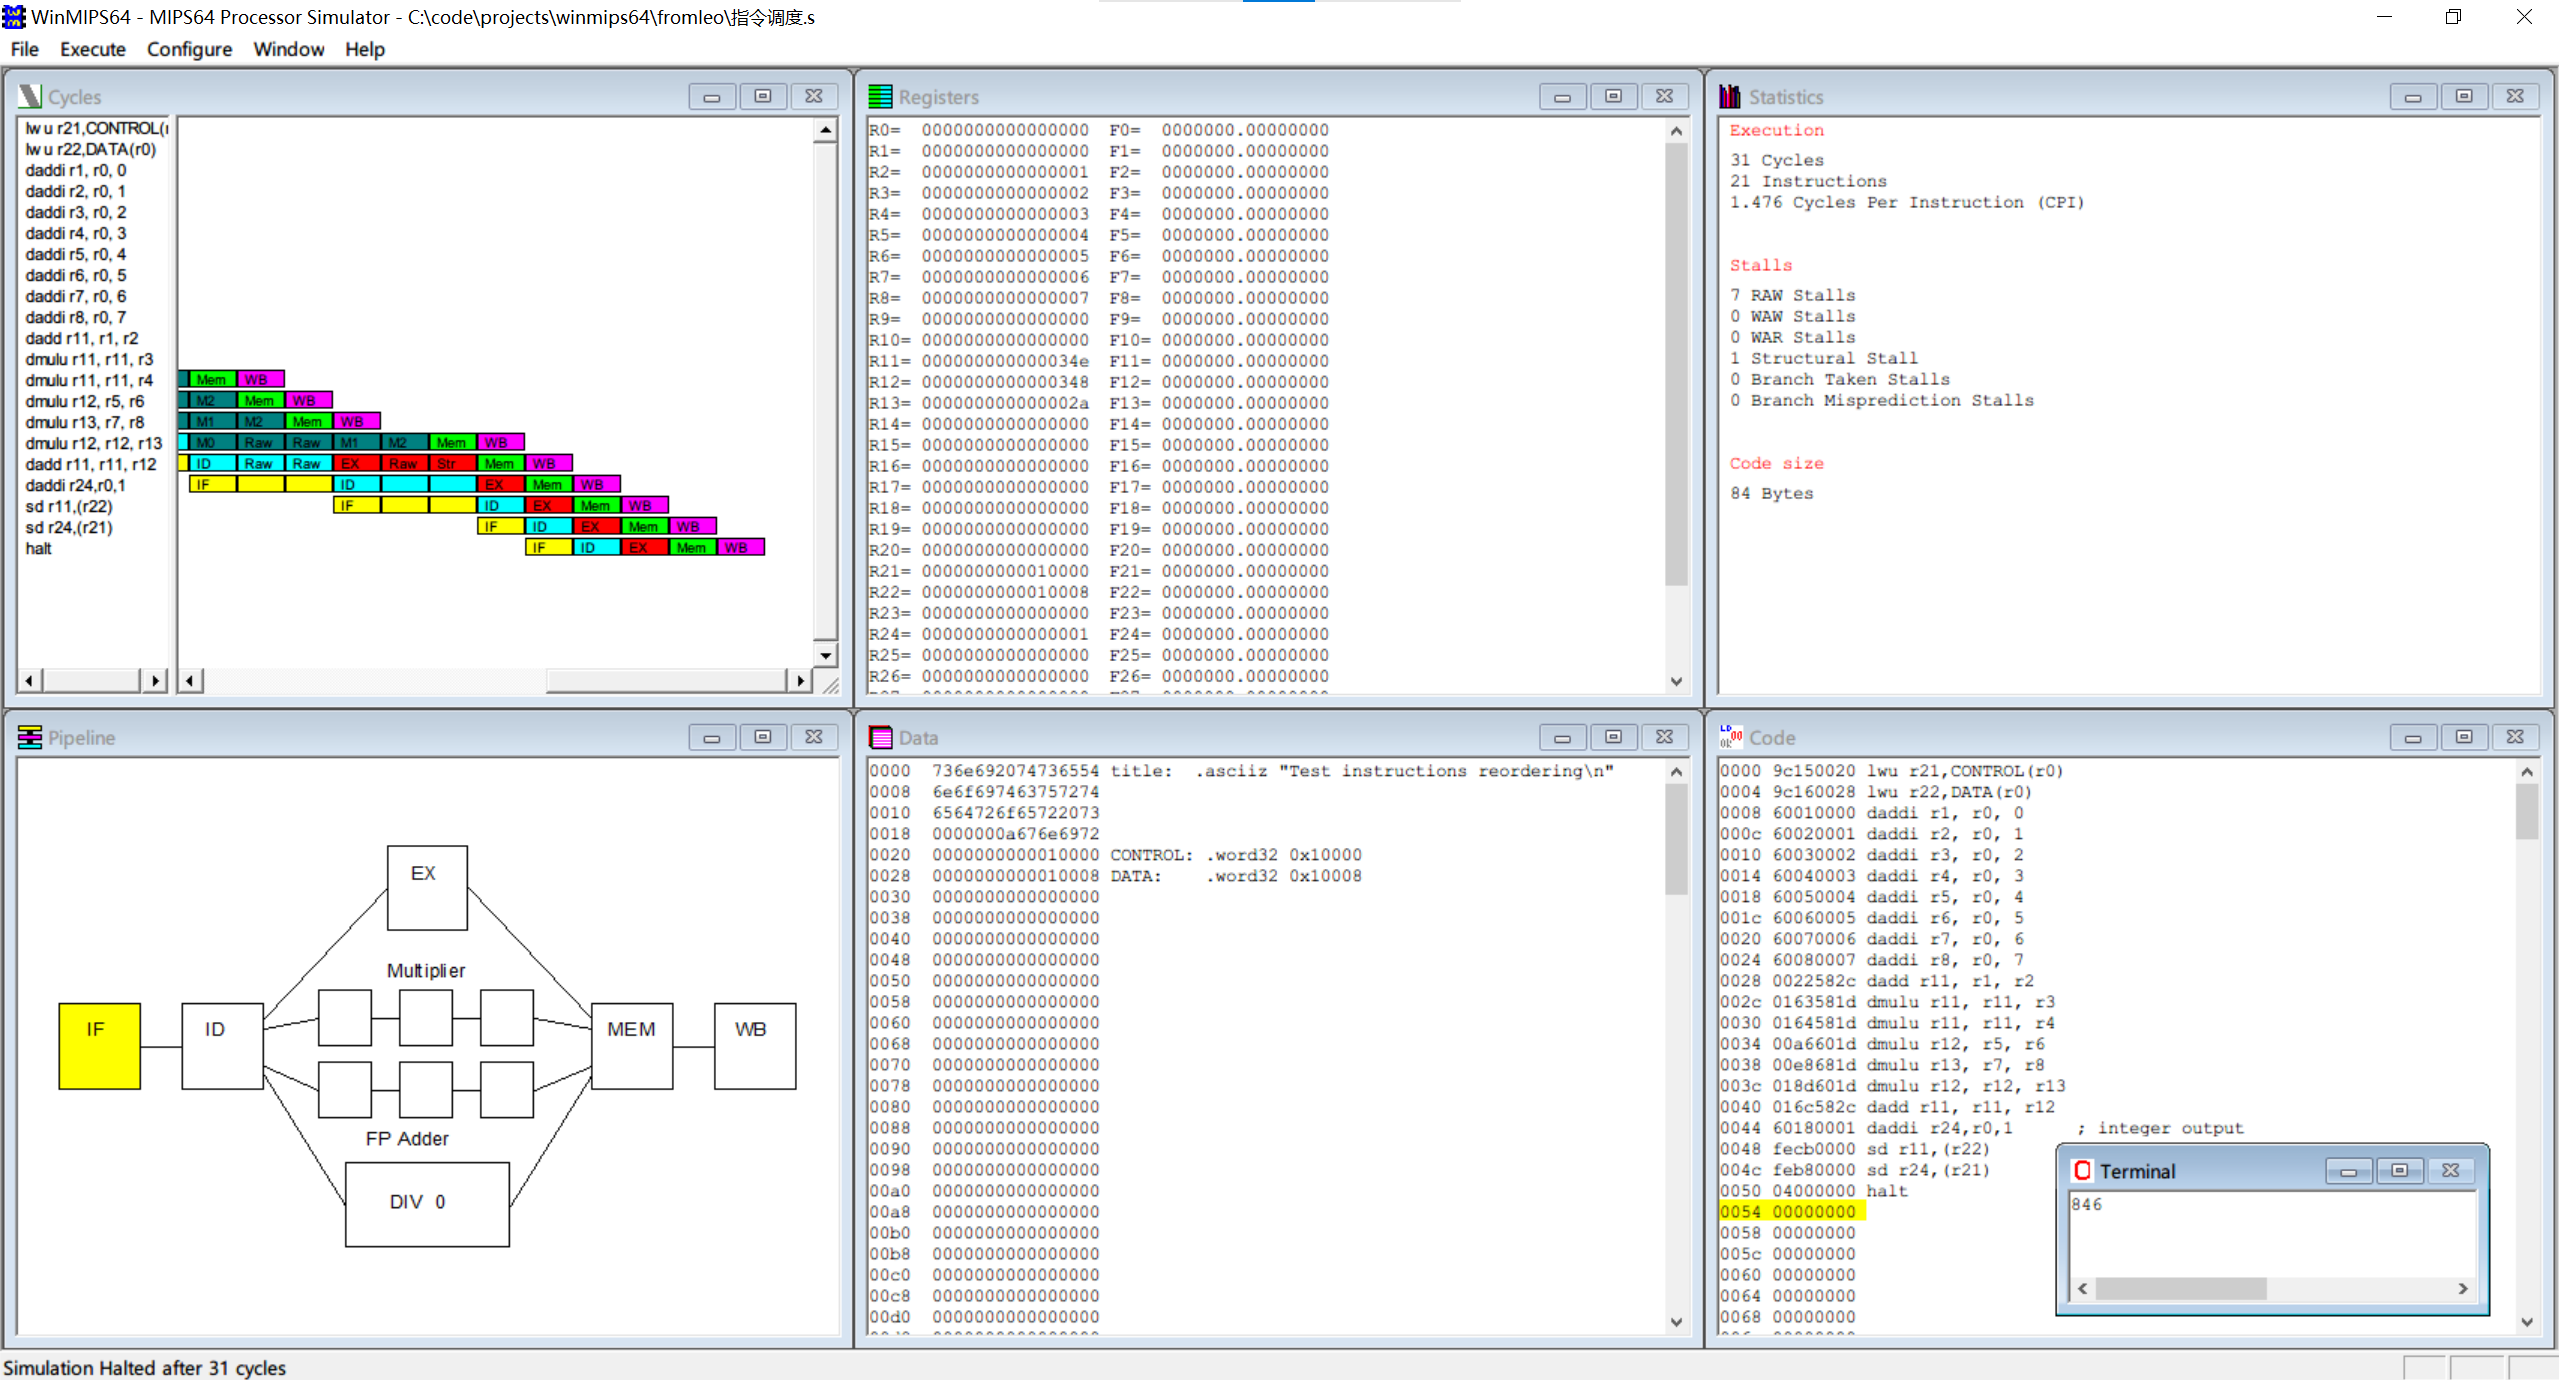
\includegraphics[width=\linewidth]{instruction-reordering-before}
        \caption{指令调度之前的运行结果}
    \end{subfigure}
    \begin{subfigure}{.8\linewidth}
        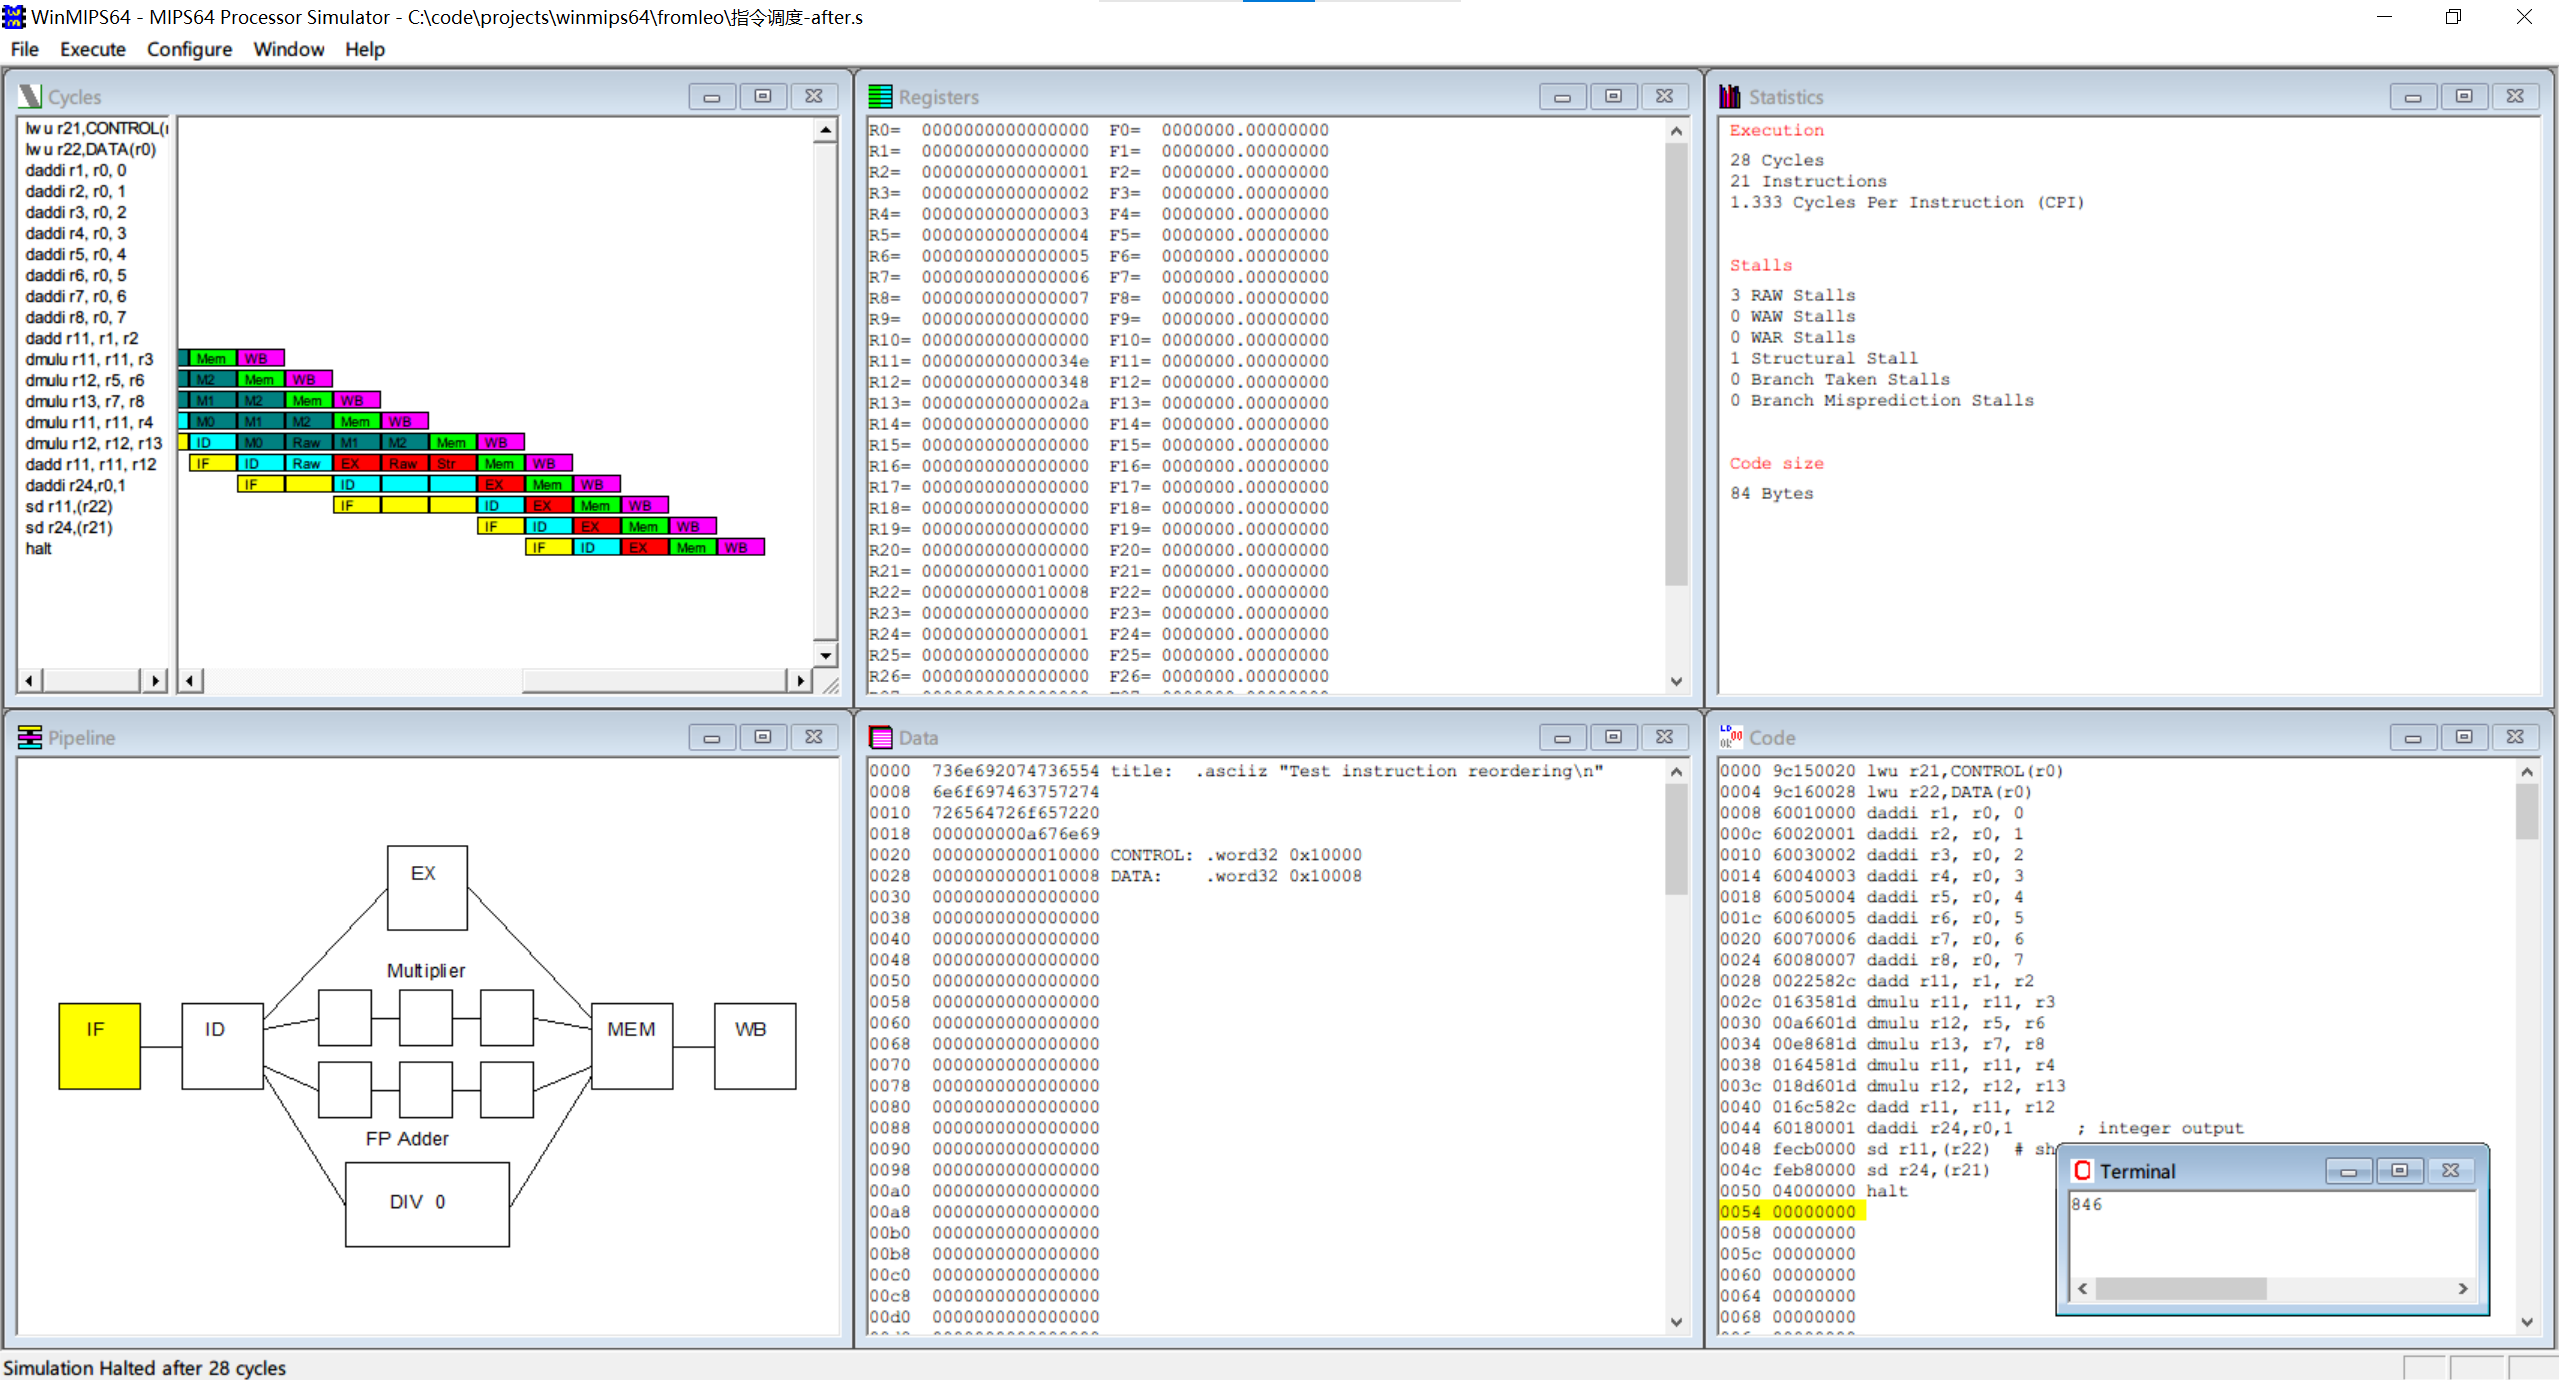
\includegraphics[width=\linewidth]{instruction-reordering-after}
        \caption{指令调度之后的运行结果}
    \end{subfigure}
    \caption{指令调度运行结果}
    \label{fig:ir}
\end{figure}

程序运行结果见\fullref{fig:ir}。可以看到,运行结果相同,减少了4个先读后写的数据相关,加速了3个周期,同时执行结果正确,意味着指令重排前后程序逻辑一致。

\subsection{循环展开、寄存器换名以及指令调度提高性能}

\subsubsection{测试程序}

循环展开使用的测试程序为计算fibonacci数列的第32项,代码如下:
\begin{minted}[linenos,breaklines]{gas}
        .data
title:  .asciiz "Test loop unrolling\n"

CONTROL: .word32 0x10000
DATA:    .word32 0x10008

.text

lwu r21,CONTROL(r0)
lwu r22,DATA(r0)
daddi r24,r0,4      ; ascii output
daddi r1,r0,title   
sd r1,(r22)
sd r24,(r21)

daddi r11, r0, 0 ; f0 = 0
daddi r12, r0, 1 ; f1 = 1


daddi r10, r0, 32 ; loop 30 times
loop:
dadd r13, r12, r11 ; r13 = r12 + r11

dadd r11, r0, r12 ; r11 = r12
dadd r12, r0, r13 ; r12 = r13
daddi r10, r10, -1 ; r10 -= 1

bnez r10, loop

daddi r24,r0,1      ; integer output
sd r11,(r22)
sd r24,(r21)

halt
\end{minted}

代码存在先读后写数据相关与控制语句。展开循环3次、寄存器换名、指令重排后的代码如下:

\begin{minted}[linenos,breaklines]{gas}
        .data
title:  .asciiz "Test loop unrolling\n"

CONTROL: .word32 0x10000
DATA:    .word32 0x10008

.text

lwu r21,CONTROL(r0)
lwu r22,DATA(r0)
daddi r24,r0,4      ; ascii output
daddi r1,r0,title   
sd r1,(r22)
sd r24,(r21)

daddi r11, r0, 0 ; f0 = 0
daddi r12, r0, 1 ; f1 = 1


daddi r10, r0, 32 ; loop 30 times
loop:
# dadd r13, r12, r11 ; r13 = r12 + r11

# dadd r11, r0, r12 ; r11 = r12
# dadd r12, r0, r13 ; r12 = r13
# daddi r10, r10, -1 ; r10 -= 1

dadd r13, r12, r11
dadd r14, r12, r13
dadd r15, r13, r14
dadd r16, r14, r15


daddi r10, r10, -4

dadd r11, r0, r15
dadd r12, r0, r16


bnez r10, loop

daddi r24,r0,1      ; integer output
sd r11,(r22)
sd r24,(r21)

halt
\end{minted}

通过循环展开3次,可以在执行过程中减少75\%的循环控制语句,达到加速执行的目的。同时,使用指令重排技术解决了循环计数器 \gas{r10} 寄存器的先读后写数据相关。

当前程序仍有4次的条件跳转等待,可以通过延迟槽技术解决:

\begin{minted}[linenos,breaklines]{gas}
        .data
title:  .asciiz "Test loop unrolling\n"

CONTROL: .word32 0x10000
DATA:    .word32 0x10008

.text

lwu r21,CONTROL(r0)
lwu r22,DATA(r0)
daddi r24,r0,4      ; ascii output
daddi r1,r0,title   
sd r1,(r22)
sd r24,(r21)

daddi r11, r0, 0 ; f0 = 0
daddi r12, r0, 1 ; f1 = 1


daddi r10, r0, 32 ; loop 30 times
loop:
# dadd r13, r12, r11 ; r13 = r12 + r11

# dadd r11, r0, r12 ; r11 = r12
# dadd r12, r0, r13 ; r12 = r13
# daddi r10, r10, -1 ; r10 -= 1

dadd r13, r12, r11
dadd r14, r12, r13
dadd r15, r13, r14
dadd r16, r14, r15

daddi r10, r10, -4
dadd r11, r0, r15


bnez r10, loop
dadd r12, r0, r16

daddi r24,r0,1      ; integer output
sd r11,(r22)
sd r24,(r21)

halt
\end{minted}

通过将一条循环内的计算指令移动到循环跳转指令的延迟槽中执行,可以消除掉条件跳转等待,加快程序运行速度。

程序运行结果见 \fullref{fig:lu}。可以看到,程序执行时间分别为240、88、81周期,同时执行结果正确,意味着展开前后程序逻辑一致。

\begin{figure}
    \centering
    \begin{subfigure}{0.8\linewidth}
        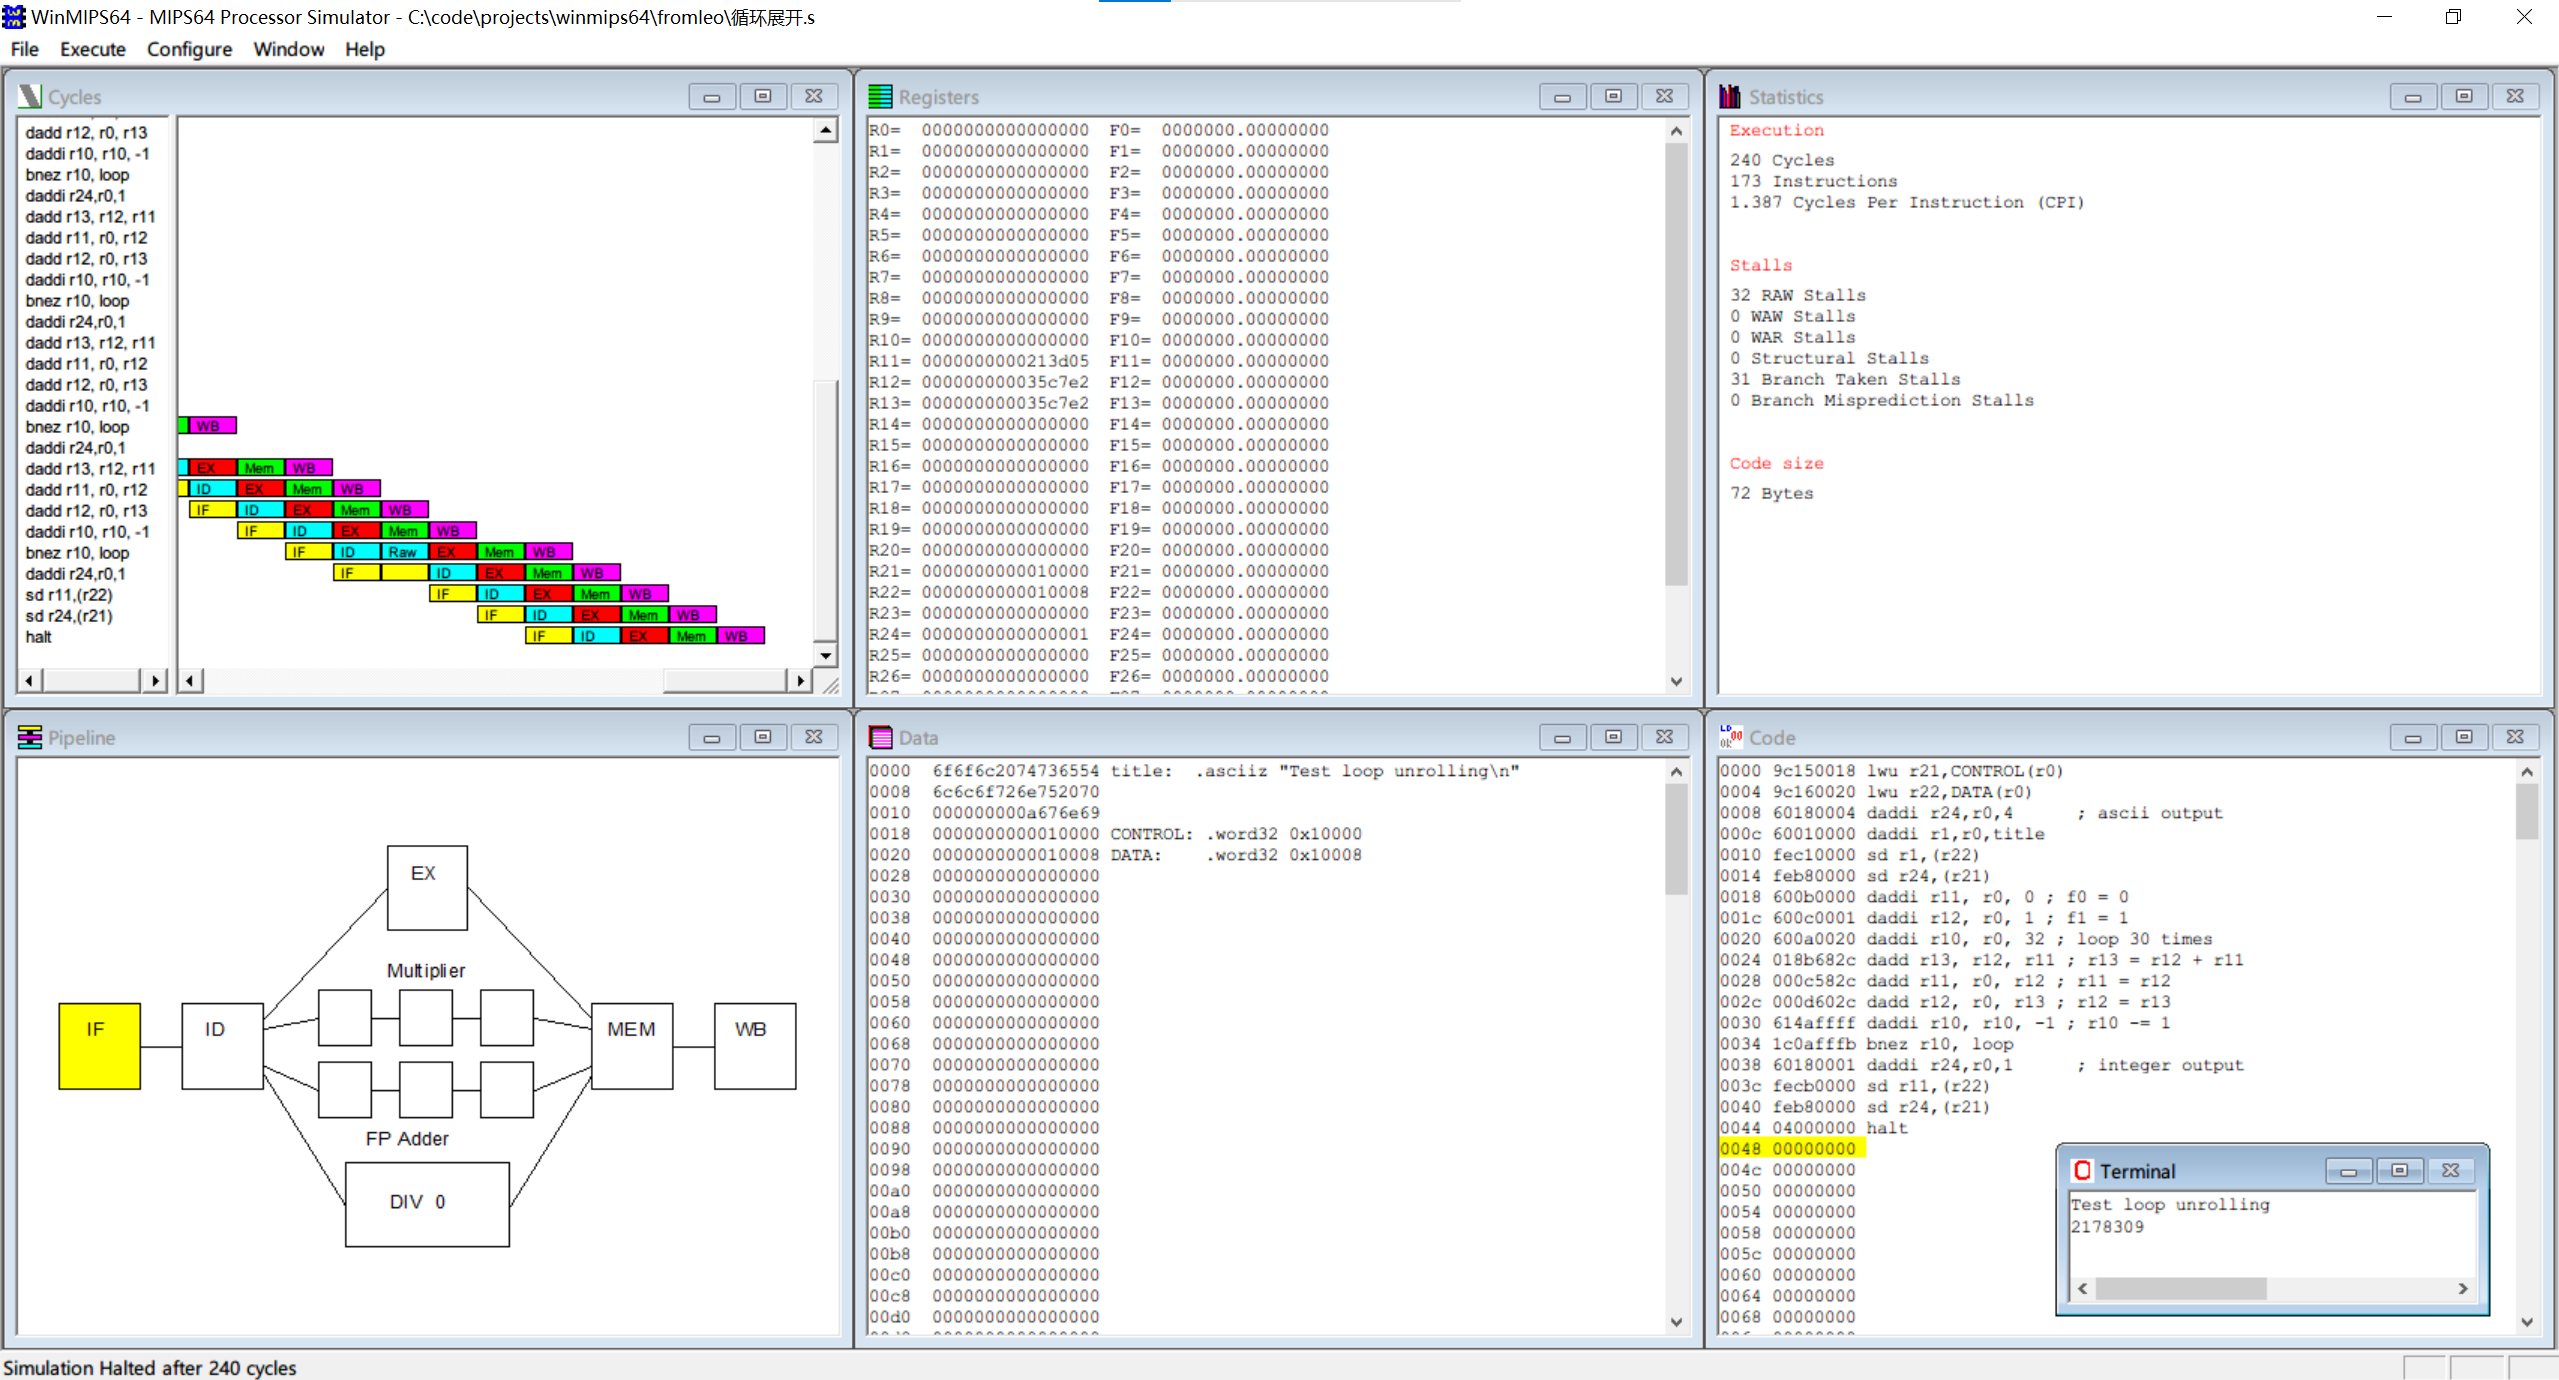
\includegraphics[width=\linewidth]{loop_unrolling_before.png}
        \caption{循环展开前的运行结果}
    \end{subfigure}
    \begin{subfigure}{0.8\linewidth}
        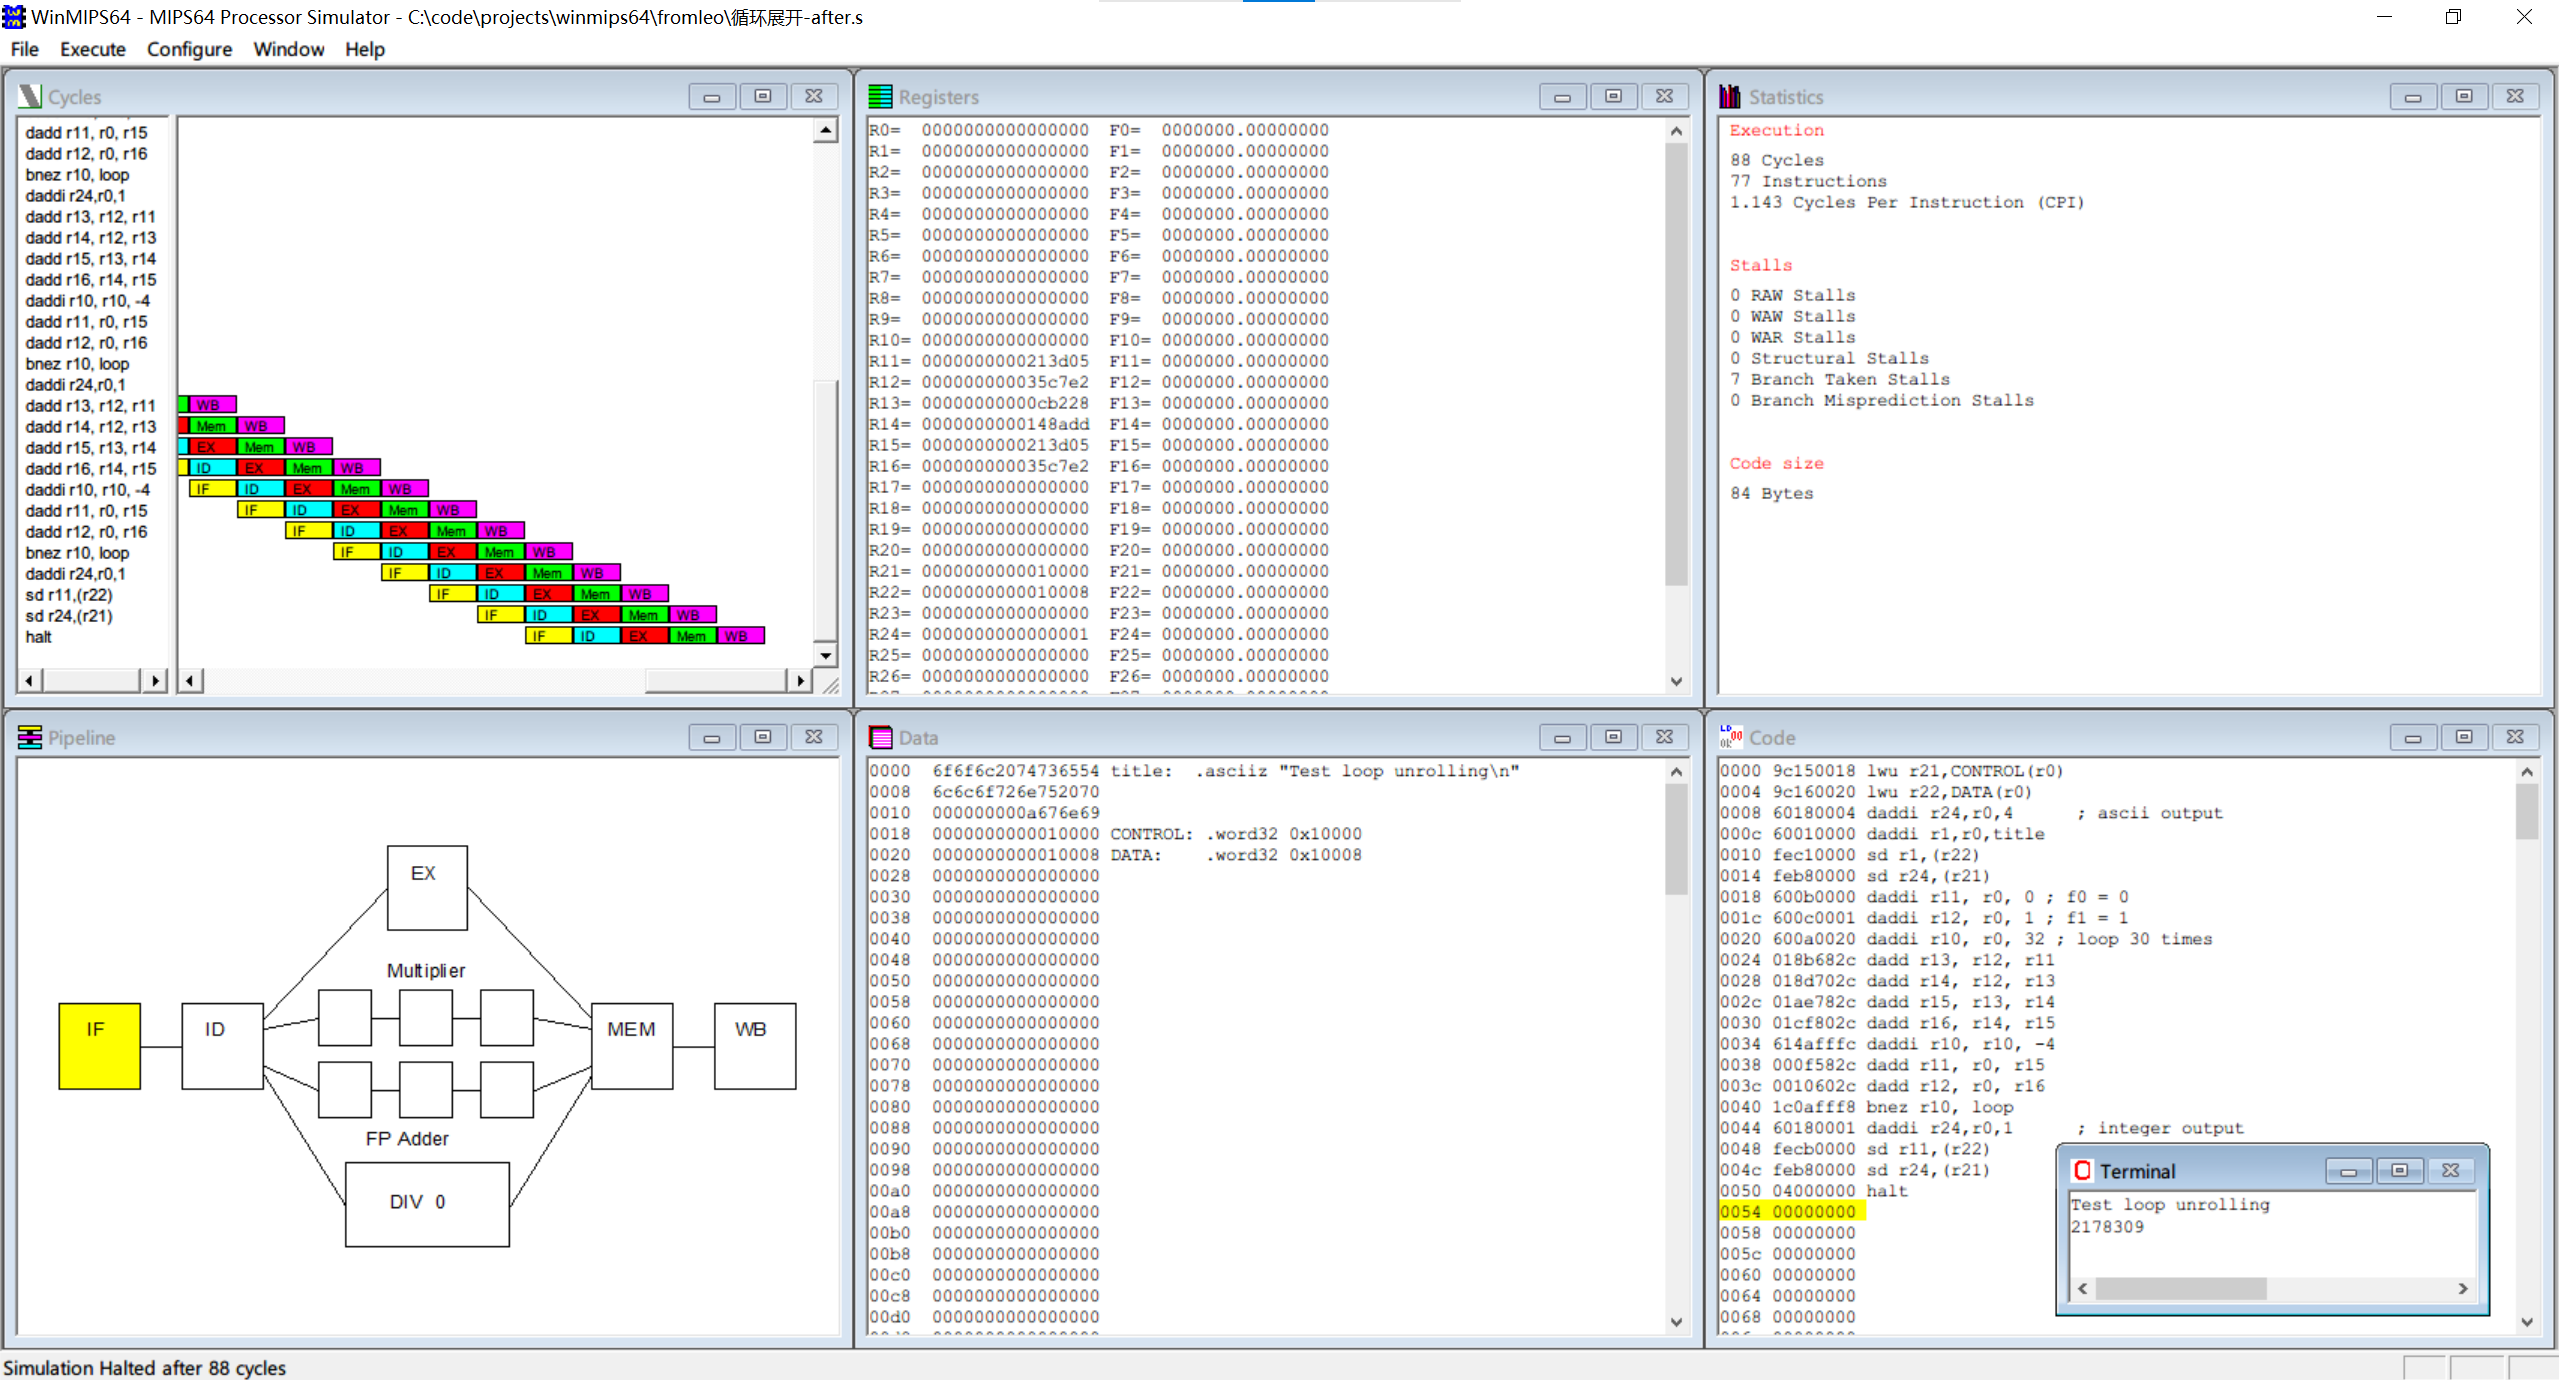
\includegraphics[width=\linewidth]{loop_unrolling_after.png}
        \caption{循环展开后的运行结果}
    \end{subfigure}
    \begin{subfigure}{0.8\linewidth}
        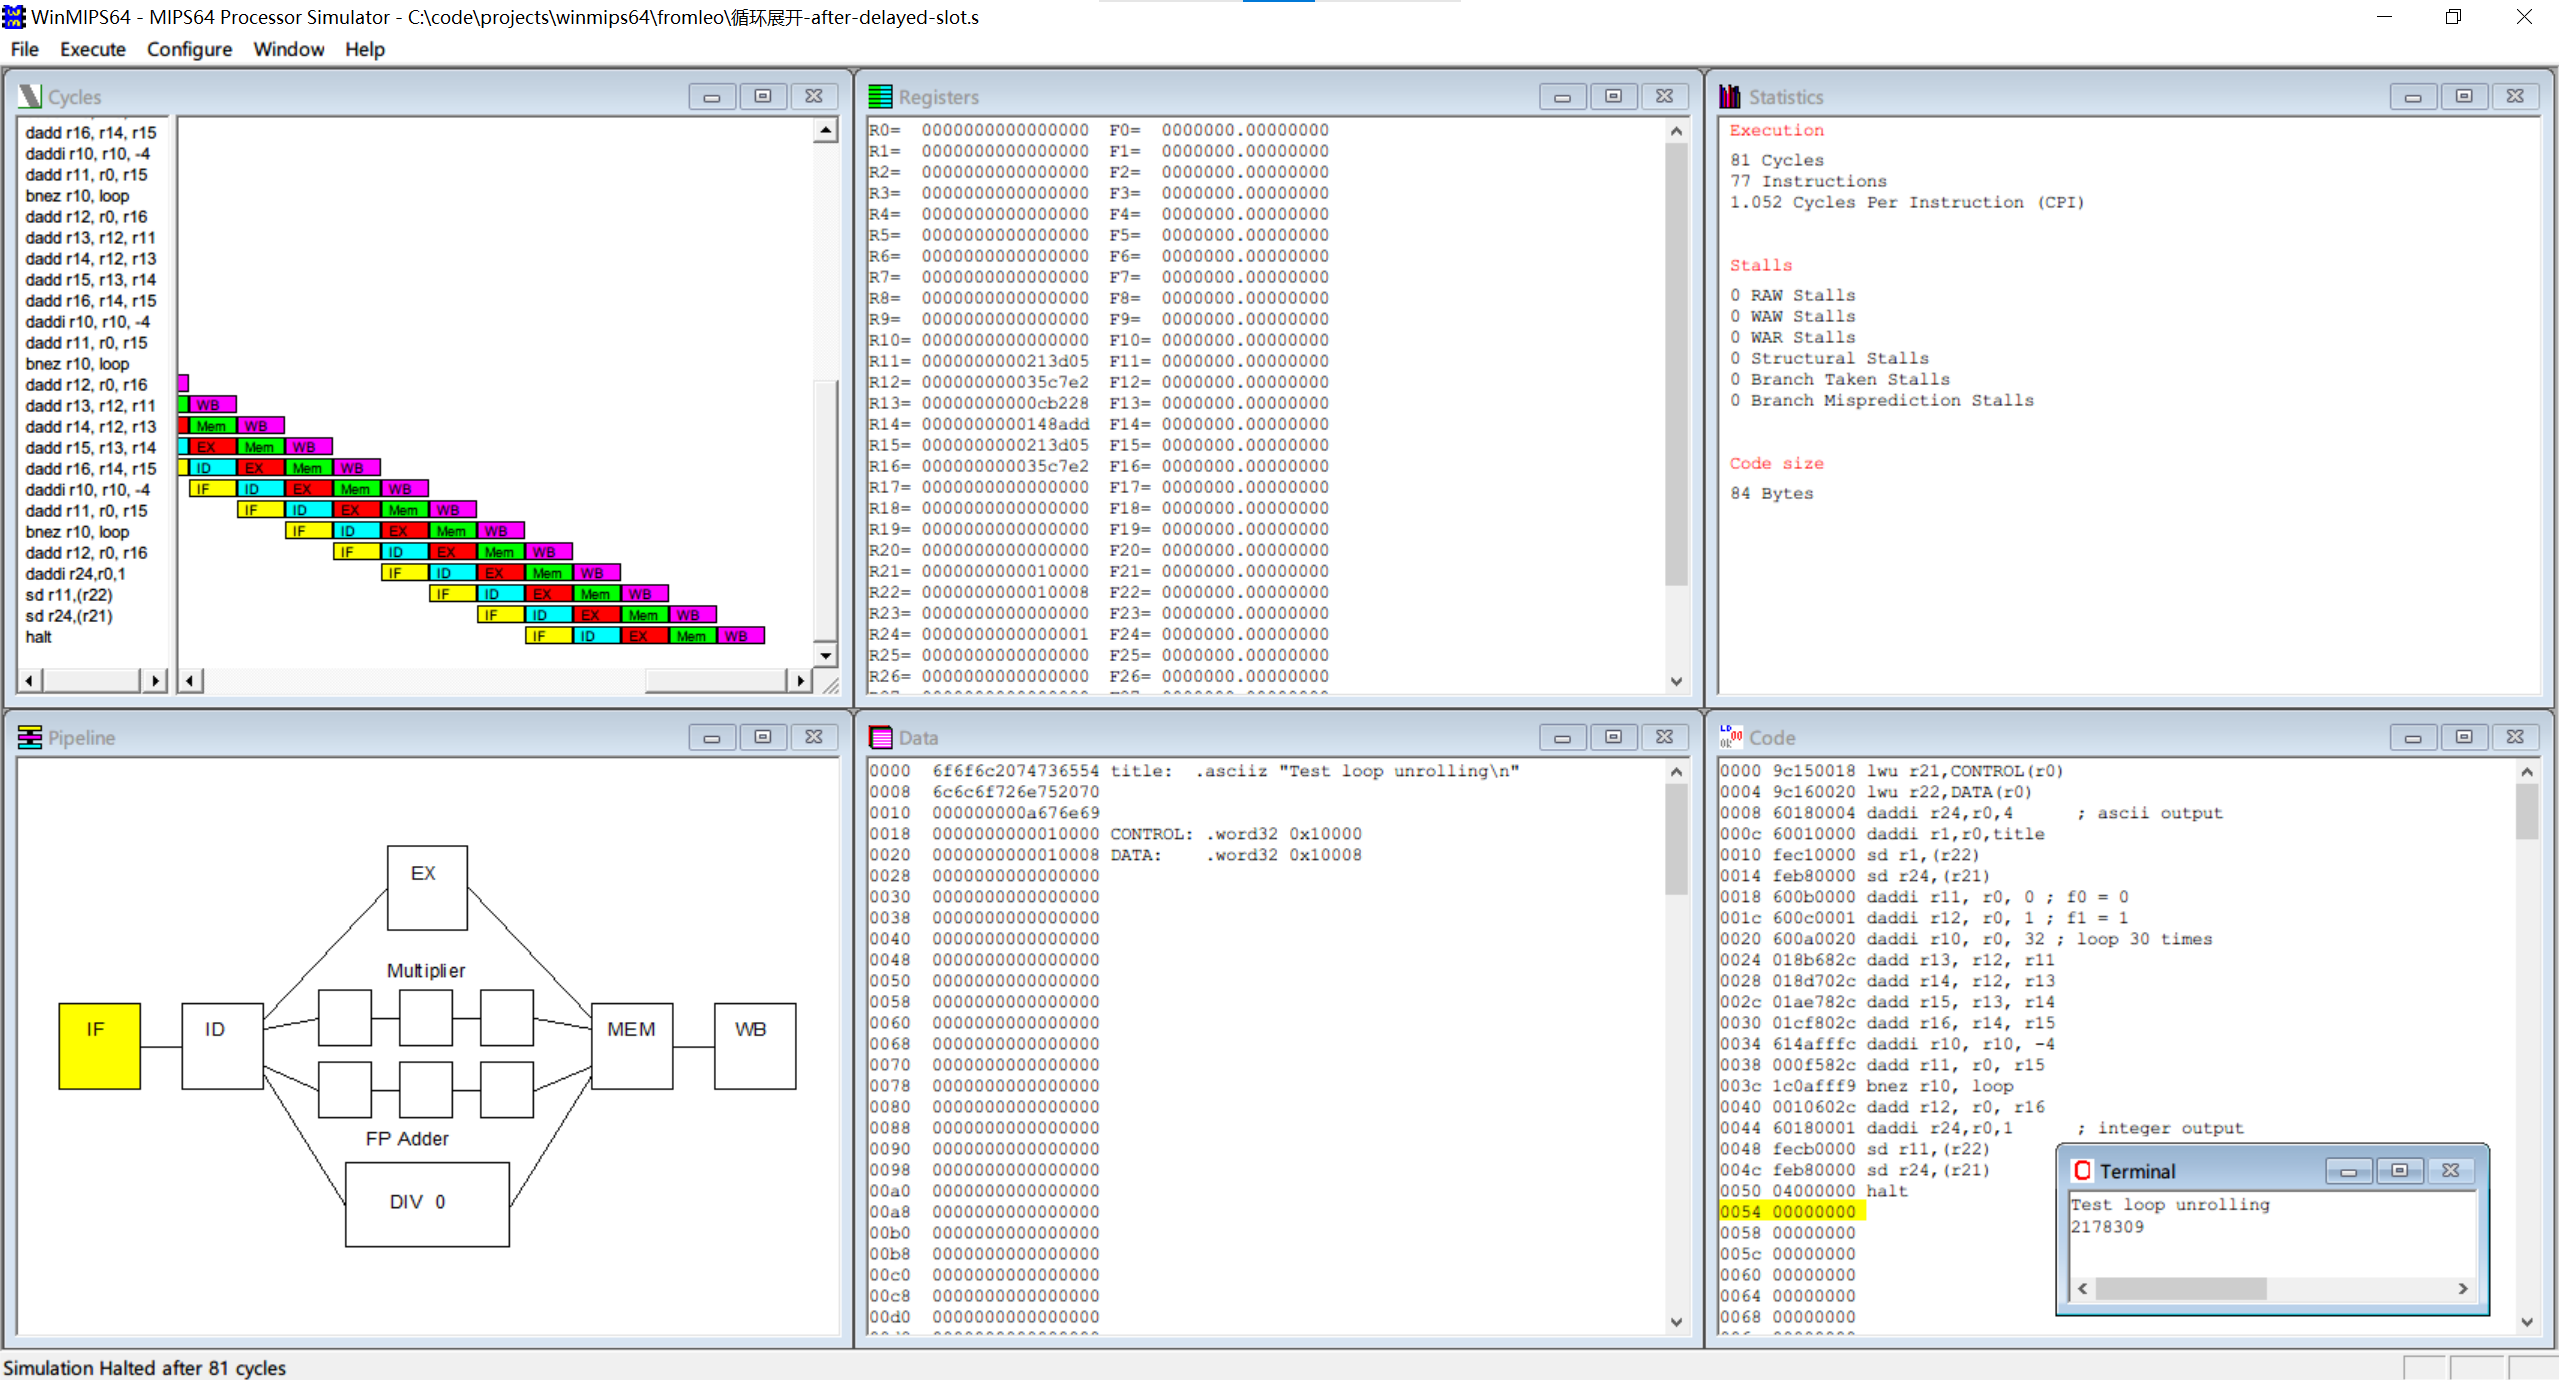
\includegraphics[width=\linewidth]{loop_unrolling_ds.png}
        \caption{循环展开后、启用延迟槽的运行结果}
    \end{subfigure}
    \caption{循环展开测试程序执行结果}
    \label{fig:lu}
\end{figure}

\section{总结与提高}

在这次实验中,我了解了各种汇编层面对于程序进行优化的方式。在高中参加信息学竞赛时,由于不开启编译器优化,我曾经简单了解过循环展开等优化方式,有的时候需要手动进行循环展开和函数内联。经过本次实验,我深入了解了循环展开等优化的原理和限制(如展开次数太多会导致寄存器不够用,从而导致效率降低)。

同时,本次实验过程中,我也了解了『过早优化是万恶之源』。在优化调整程序的过程中,多次出现优化后程序运行反而变慢或者没有变快的现象。因此,应该尽可能自动化、程序化的进行优化,这样可以避免人在优化时考虑不周全的问题,同时可以自动化的尝试多种优化方案,让执行效率最高。

在编写程序的过程中,如果需要最高效率的执行,则可采用平台特定的、深度优化的编译器,如在Intel CPU的电脑上使用icc作为编译器并开启编译优化。这样,可以使得源代码的逻辑尽可能简单,同时让编译之后的程序运行结果尽可能变高。

\chapter{Cache性能分析}
\section{实验目的}
\begin{outline}[enumerate]
    \1 加深对 Cache 的基本概念、基本组织结构以及基本工作原理的理解;
    \1 了解 Cache 的容量、相联度、块大小对Cache 性能的影响;
    \1 掌握降低 Cache 失效率的各种方法,以及这些方法对Cache 性能提高的好处;
    \1 理解 Cache 失效的产生原因以及Cache 的三种失效;
    \1 理解 LRU 与随机法的基本思想,及它们对Cache 性能的影响。
\end{outline}
\section{实验内容及步骤}
\begin{outline}[enumerate]
    \1 在基本配置情况下运行程序(请指明所选的测试程序),统计Cache 总失效次数、三种不同种类的失效次数;
    \1 改变Cache 容量(*2,*4,*8,*64),运行程序(指明所选的测试程序),统计各种失效的次数,并分析Cache 容量对Cache 性能的影响;
    \1 改变Cache 的相联度(1 路,2 路,4 路,8 路,64 路),运行程序(指明所选的测试程序),统计各种失效的次数,并分析相联度对Cache 性能的影响;
    \1 改变Cache 块大小(*2,*4,*8,*64),运行程序(指明所选的测试程序),统计各种失效的次数,并分析Cache块大小对Cache性能的影响;
    \1 分别采用LRU 与随机法,在不同的Cache容量、不同的相联度下,运行程序(指明所选的测试程序)统计Cache总失效次数,计算失效率。分析不同的替换算法对Cache性能的 影响。
\end{outline}

\section{实验方法}
\subsection{配置参数}

鉴于实验指导书中没有给出实验的初始参数,我们遍历了所有和里的参数,找到了一组实验效果较为显著的初始参数,如\fullref{tab:cache-arguments}所示。

\begin{table}[htp]
    \centering
    \begin{tabular}{cccccc}
        \toprule
        实验名称 & 参数名称 & 参数意义 & 初始值 & 合法范围 & 测试范围 \\
        \midrule
        块大小 & 块大小 & 每块的大小 & 8 & $\ge 8$ & $\times 1, \times 2, \times 4, \times 8$ \\
        相联度 & 相联度 & 每组的块数 & 2 & $\ge 2$ & $\times 1, \times 2, \times 4, \times 8, \times 16, \times 32, \times 64$ \\
        总容量 & 组数 & 组数 & 64 & $\ge 2$ & $\times 1, \times 2, \times 4, \times 8, \times 16, \times 32, \times 64$ \\
        替换算法 & 替换算法 & 替换算法 & l & l, f, r & l, f, r \\
        \bottomrule
    \end{tabular}
    \caption{Cache实验参数设置}
    \label{tab:cache-arguments}
\end{table}

\subsection{测试方法}

我们使用sim-cache对多个程序进行测试,使用脚本自动化程序运行并绘制图表。

\section{实验结果}

\subsection{块大小实验}

块大小实验结果见\fullref{fig:block-size}。可以发现,随着块大小的提升,大部分程序的缓存失效次数下降。这可以解释为,块大小提升后,根据局部性原理,程序使用一端数据时,附近更多的数据被一起缓存了,使得使用附近的数据时不需要再去主存加载,使得失效次数降低。

对于失效次数先下降再上升的情况,我们认为这两个程序的内存访问模式和其他程序不太相同,访问的数据更为分散。块大小提升时,首先由于一次性缓存的数据更多使得缓存效率提升;然后则由于程序访问内存非常分散,而块大小提升后块的数量减少了,也就意味着无法处理分散的内存访问,失效次数提高。

\figroup{dl1-块大小实验结果}{fig:block-size}
{(1, 1993.0) (2, 1225.0) (4, 910.0) (8, 801.0)}{(1, 1767.0) (2, 921.0) (4, 503.0) (8, 327.0)}{(1, 1708.0) (2, 881.0) (4, 461.0) (8, 272.0)}{(1, 3695.0) (2, 2738.0) (4, 2723.0) (8, 2819.0)}{(1, 13703.0) (2, 11862.0) (4, 12069.0) (8, 14020.0)}


\subsection{相联度实验}

相联度试验结果见\fullref{fig:association-ratio}。相联度即组内块数,在相联度实验中,我们为了控制变量,在增大块数的同时减少了总的组数以保证缓存总大小不变。

观察试验结果可以发现,随着相联度的提升,所有程序的命中率均显著提升。这是因为,由于采用组相连算法,组内全相连,即可以缓存内存中任意位置的数据,而组间采用直接相连,即只能缓存固定区域的内存。提升相联度,意味着每一块缓存可以对应更多的内存地址,即分配更为灵活。这就有效的提升了缓存的利用率,使得失效次数降低。

\figroup{dl1-相联度实验结果}{fig:association-ratio}
{(1, 1993.0) (2, 1943.0) (4, 1905.0) (8, 1896.0) (16, 1858.0) (32, 1856.0) (64, 1856.0) }{(1, 1767.0) (2, 1751.0) (4, 1745.0) (8, 1740.0) (16, 1739.0) (32, 1739.0) (64, 1740.0) }{(1, 1708.0) (2, 1707.0) (4, 1706.0) (8, 1706.0) (16, 1706.0) (32, 1706.0) (64, 1706.0) }{(1, 3695.0) (2, 3368.0) (4, 3019.0) (8, 2966.0) (16, 2962.0) (32, 2976.0) (64, 2888.0) }{(1, 13703.0) (2, 7208.0) (4, 5623.0) (8, 5317.0) (16, 5140.0) (32, 5138.0) (64, 5106.0) }


\subsection{总容量实验}

总容量试验结果见\fullref{fig:capacity}。由图可见,随着总容量增大,程序的缓存失效率基本都下降,可以看出缓存容量更大后可以缓存更多数据,自然失效次数更少。

对于极小部分情况,缓存提升失效率并没有显著下降,甚至轻微上升,则是因为那些程序拥有较为特殊的内存访问模式。在数学上可以证明在全相联、使用LRU算法时没有Belady异常,即随着缓存大小的提升,缓存命中率一定提升。但是,实际使用的是组相联,使得LRU算法在极小数情况下也会产生Belady异常。

\figroup{dl1-总容量实验结果}{fig:capacity}
{(1, 1993.0) (2, 1850.0) (4, 1819.0) (8, 1819.0) (16, 1803.0) (32, 1762.0) (64, 1762.0) }{(1, 1767.0) (2, 1743.0) (4, 1741.0) (8, 1741.0) (16, 1696.0) (32, 1689.0) (64, 1689.0) }{(1, 1708.0) (2, 1706.0) (4, 1706.0) (8, 1706.0) (16, 1663.0) (32, 1657.0) (64, 1657.0) }{(1, 3695.0) (2, 2505.0) (4, 2278.0) (8, 2093.0) (16, 2017.0) (32, 1998.0) (64, 1998.0) }{(1, 13703.0) (2, 6277.0) (4, 3859.0) (8, 2704.0) (16, 2558.0) (32, 2542.0) (64, 2542.0) }


\subsection{替换方法实验}

替换方法实验结果见\fullref{fig:replace}。大多数情况下,LRU、FIFO、Random的效果依次变差。因为,这三种算法中,LRU、FIFO都不同程度上考虑了程序的内存访问模式,而Random完全不考虑。LRU认为,很久没用到的内存就不会再用了,某种意义上更符合现实的现象,也更符合局部性原理。FIFO认为,程序每块内存只会访问一小段时间,和现实中程序访问内存的逻辑更为不符合。

\figroupstr{dl1-替换方法实验结果}{fig:replace}
{(l, 1993.0) (f, 2018.0) (r, 2051.0) }{(l, 1767.0) (f, 1769.0) (r, 1779.0) }{(l, 1708.0) (f, 1708.0) (r, 1717.0) }{(l, 3695.0) (f, 3923.0) (r, 4001.0) }{(l, 13703.0) (f, 14884.0) (r, 14877.0) }

\section{总结与提高}

经过本次实验,我印证了系统结构和操作系统课程中学到的程序局部性原理等规则,也充分理解了缓存的各个参数的意义以及对与缓存效率的影响。

在真正设计CPU的时候,要考虑到不同程序的内存访问模式。如,Intel最新的服务器系列CPU就提供了搜索引擎优化、数据库优化等不同的版本。只有综合了目标程序的特点,选择对应的参数和算法,才能让整体执行效率最高。

\end{document}
